\documentclass{pjatk}

\usepackage{tocloft}
\usepackage{hyperref}
\usepackage[english,polish]{babel}
\usepackage{tikz-uml}
\usepackage[acronym, toc]{glossaries}

\addbibresource{attachments/bibliography.bip}

\makeglossaries
%! Author = Mateusz Budzisz
%! Date = 08/11/2023

\newglossaryentry{pwa}{name={Progressive Web App},
description={Progressive Web App (PWA) to progresywna aplikacja internetowa uruchamiana tak jak zwykła strona internetowa,
 ale umożliwiająca stworzenie wrażenia działania jak natywna aplikacja mobilna lub aplikacja desktopowa. }
}
\newglossaryentry{aws}{name={Amazon Web Services},
description={Amazon Web Services (AWS) – pakiet usług chmurowych oferowanych przez Amazon},
}
\newglossaryentry{gcp}{name={Google Cloud Platform},
description={Oferowany przez Google zestaw usług chmurowych, obejmuje szereg modułowych usług chmurowych, w tym przetwarzanie danych, przechowywanie danych, analitykę danych oraz uczenie maszynowe, a także zestaw narzędzi zarządzania.}
}
\newglossaryentry{azure}{ name={Azure},
description={Microsoft Azure to platforma chmurowa firmy Microsoft stworzona w modelu PaaS (Platform as a Service)}
}
\newglossaryentry{osm}{name={Open Street Map},
description={OpenStreetMap (OSM) – projekt społeczności internetowej mający na celu stworzenie darmowej, swobodnie dostępnej mapy całej kuli ziemskiej.}}
\newglossaryentry{lsp}{name={Language Service Protocol},
description={Protokół Language Server Protocol (LSP) to otwarty protokół oparty na JSON-RPC, stosowany pomiędzy edytorami kodu źródłowego lub zintegrowanymi środowiskami programistycznymi (IDE) a serwerami, które dostarczają "narzędzia inteligencji językowej": specyficzne dla języków programowania funkcje, takie jak uzupełnianie kodu, podświetlanie składni oraz oznaczanie ostrzeżeń i błędów, a także rutyny refaktoryzacji.}
}
\newglossaryentry{osw}{
name={Open Weather Map},
description={Open Weather Ma} 
}
\newglossaryentry{http}{name={Hyper Text Transfer Protocol},
description={ Hyper Text Transfer Protocol protokół stworzony przez Tima Bernersa-Lee na potrzeby komunikacji między klientem a serwerem w sieci WWW (ang. World Wide Web).}
}

\newglossaryentry{drag-n-drop}
{
    name={Drag and drop},
    description={Technologia umożliwiająca interfejsom użytkownika w przeglądarkach internetowych korzystanie z funkcji przeciągania i upuszczania elementów. Użytkownik może wybrać elementy do przeciągania za pomocą myszy, przeciągnąć te elementy do elementu docelowego i upuścić je, zwalniając przycisk myszy. Podczas operacji przeciągania półprzezroczysta reprezentacja przeciąganych elementów podąża za wskaźnikiem myszy.}
}

\newglossaryentry{on-demand}
{
    name={On-demand},
    description={Rodzaj oprogramowania charakteryzującego się dynamicznym czasem pracy, uruchamiane na rządanie, gdy poda wynik program kończy pracę zamiast oczekiwać następnego zapytania}
}

\newglossaryentry{refactoring}
{
    name={Refactoring},
    description={Znaczna zmiana konstrukcji programu mająca na celu usprawnienie oprogramowania bądź dostosowanie go do nowych wymogów}
}

\newglossaryentry{ui}
{
    name={UI},
    description={Interfejs użytkownika}
}

\newglossaryentry{frontend}
{
    name={Frontend},
    description={Oprogramowanie składające się z UI z którym docelowy użytkownik będzę wchodził w interakcję}
}

\newglossaryentry{backend}
{
    name={Backend},
    description={Oprogramowanie pozbawione UI z którym docelowy użytkownik będzę wchodził w interakcję, potrzebne do prawidłowej pracy Frontendu}
}

\newglossaryentry{job}
{
    name={Job},
    description={Oprogramowanie, które ma z góry określony cel, po jego uruchomieniu natychmiast zaczyna je wykonywać, nie wchodzi w interakcje z użytkownikiem docelowym, po zakończeniu kończy swoje życie}
}


\newglossaryentry{rendering}
{
    name={Wyrenderowanie},
    description={Stworzenie UI z postaci kodu do postaci konsumowalnej przez użytkownika docelowego}
}

\newglossaryentry{hello-world}
{
    name={Hello world},
    description={Minimalny reprezentatywny program w danej technologii}
}

\newglossaryentry{hermetyzacja}
{
    name={Hermetyzacja},
    description={Hermetyzacja opgorgramowania określa dobrą praktykę programistyczną polegającą na izolacji komponentów w aplikacji tak aby o sobie nie wiedziały gdy nie muszą o sobie wiedzieć}
}

\newglossaryentry{infra-as-code}
{
    name={Infrastructure as a code},
    description={Sposób opisania architektury systemu poprzez napisanie programu tworzącego docelową architekturę przy pomocy abstrakcji dostarczonych przez dostawcę mocy obliczeniowej}
}

\newglossaryentry{on-prem}
{
    name={On-premise},
    description={Oprogramowanie hostowane na samodzielnie zarządzanej infrastrukturze}
}

\newglossaryentry{virt}
{
    name={Wirtualizacja},
    description={Podział serwera na maszyny o mniejszej mocy obliczeniowej, aby umożliwić podział podzespołów pomiędzy klientów tak, aby nic o sobie nawzajem nie wiedzieli}
}

\newglossaryentry{arm}
{
    name={Architektura ARM},
    description={Architektura silnej ręki lol}
}
\newglossaryentry{poidef}
{
    name={POI},
    description={Point of interest (w skrócie POI) to punkt w przestrzeni, najczęściej na powierzchni Ziemi.}
}
\newglossaryentry{openlayers}
{
    name={Openlayers},
    description={OpenLayers to biblioteka napisana w języku JavaScript, ułatwiająca dodawanie dynamicznych map na stronach internetowych.}
}
\newglossaryentry{reflink}
{
    name={Reflink},
    description={Reflink to specjalny link, który zawiera unikalny kod identyfikacyjny, pozwalający na monitorowanie ruchu i przekierowań z innych źródeł.}
}
\newglossaryentry{sla}
{
    name={SLA},
    description={Service Level Agreement, SLA (umowa o gwarantowanym poziomie świadczenia usług) to umowa utrzymania i systematycznego poprawiania ustalonego między usługodawcą a usługobiorcą poziomu jakości usług poprzez stały cykl obejmując: uzgodnienia,
    monitorowanie usługi, raportowanie, przegląd osiąganych wyników.}
}
\newglossaryentry{sws}
{
    name={SWS},
    description={Specyfikacja Wymagań Systemowych }
}
\newglossaryentry{moscow}
{
    name={MoSCoW},
    description={Metoda MoSCoW to technika priorytetyzacji wykorzystywana w analizie biznesowej i przy tworzeniu oprogramowania w celu osiągnięcia wspólnego zrozumienia pomiędzy interesariuszami co do znaczenia, jakie ma dla nich dostarczenie każdego z wymagań. Inne nazwy metody to priorytetyzacja MoSCoW lub analiza MoSCoW.}
}
\newglossaryentry{CRUD}
{
    name={CRUD},
    description={CRUD (od angielskiego create, read, update, delete, tłumaczenie utwórz, odczytaj, aktualizuj, usuń) – cztery podstawowe funkcje w aplikacjach korzystających z bazy danych, które umożliwiają zarządzanie nią.}
}
\newglossaryentry{stadiamaps}
{
    name={Stadia Maps},
    description={Stadia Maps oferuje komercyjne interfejsy API do mapowania i wyznaczania tras, głównie oparte na OpenStreetMap.}
}

\newglossaryentry{mevo}
{
    name={Mevo},
    description={Mevo to system bezobsługowych wypożyczalni rowerów miejskich.}
}
\newglossaryentry{scraping}
{
    name={Web scraping},
    description={Data scraping to technika ekstrakcji danych z witryn internetowych.}
}
\newglossaryentry{lighthouse}
{
    name={Lighthouse},
description={Lighthouse to narzędzie open-source stworzone przez Google do automatycznego audytu stron internetowych. Analizuje wydajność, dostępność, zgodność z progresywnymi aplikacjami webowymi (PWA), SEO i najlepszymi praktykami. Wyniki audytów pomagają poprawić jakość i funkcjonalność stron internetowych. Narzędzie można uruchomić z poziomu Chrome DevTools, jako rozszerzenie Chrome lub z wiersza poleceń.}
}
\newglossaryentry{openmeteo}
{
    name={OpenMeteo},
description={OpenMeteo to darmowa, otwarta usługa dostarczająca prognozy pogody poprzez interfejs API. Oferuje precyzyjne prognozy dla różnych lokalizacji na świecie, umożliwiając integrację z aplikacjami i serwisami internetowymi.}
}


\studfield{Informatyka}
\studtype{Zaoczne}
\title{Planer Mapy Miejskiej}
\engtitle{City Map Planner}
\acronym{City Planner}
\titledate{2023-10-14}
\supervisor{prof. dr hab. Marek A. Bednarczyk}
\author{Mateusz Budzisz}{s24048}{Aplikacje Internetowe}{Zaoczny}
\author{Wiktor Rostkowski}{s23141}{Aplikacje Internetowe}{Zaoczny}
\author{Sebastian Kreft}{s23133}{Aplikacje Internetowe}{Zaoczny}
\author{Damian Kreft}{s23447}{Aplikacje Internetowe}{Zaoczny}
\consultant{--- brak ---} % Koniecznie trzeba podać brak, albo wpisać konsultantów tak jak przy autorach
\projectgoals{Stworzenie interaktywnej mapy miejskiej do planowania zwiedzania atrakcji turstycznych z wkykorzystaniem dynamicznych danych}
\productsandservices{Aplikacja progresywana}
\mainfunctionalities{Planowanie trasy}
\successmeasure{Wdrożenie rozwiązania jako oficjalnego rozwiązania miejskiego}
\projlimitations{Brak budżetu}
\date{\today}
\nabstract{
	Praca zakłada utworzenie interaktywnej mapy z punktami zainteresowań na podstawie listy atrakcji turystycznych wyróżnionych przez urząd miejski,
	umożliwiającej kompleksowe zaplanowanie optymalnej trasy zwiedzania z uwzględnieniem środków komunikacji miejskiej,
	godzin otwarcia atrakcji turystycznych oraz warunków pogodowych.
}

\graphicspath {{attachments/}}

\begin{document}

	% PJATK Template begin
	\maketitle
	\makeprojectcard
	\makedeclaration
	% PJATK Template End

	\tableofcontents
	\clearpage
	\include{chapters/przykłady-latex}
	%! Author = Wiktor Rostkowski
%! Date = 29/04/2024

%! Author = Wiktor Rostkowski, Mateusz Budzisz
%! Date = 29.10.2023

\chapter{Wstęp}
\label{ch:wstep}

W miastach, które oferują wiele atrakcji turystycznych oraz posiadają rozbudowane~i~złożone systemy transportu publicznego, tworzenie optymalnego planu zwiedzania może~być~skomplikowane~i~czasochłonne.
Konieczność uwzględnienia godzin otwarcia poszczególnych miejsc, dostępności różnych środków transportu oraz efektywnego wykorzystania czasu sprawia,~że~planowanie wycieczki wymaga dużej precyzji~i~uwagi.
Co więcej, uwzględnienie indywidualnych preferencji turystów, takich~jak~zainteresowania, tempo zwiedzania~czy~potrzeba przerw~na~odpoczynek, jeszcze bardziej zwiększa stopień trudności tego zadania.

Zespół projektowy wcześniej napotkał dokładnie~ten~problem,~co~doprowadziło~do~powstania pomysłu~na~stworzenie nowatorskiej aplikacji.
Aplikacja~ta~składa~się~z interaktywnej mapy, która prezentuje różnorodne atrakcje turystyczne~w~danym mieście, oraz kalendarza~w~stylu \gls{drag-n-drop}, umożliwiającego łatwe planowanie dnia.
Aplikacja uwzględnia dane~w~czasie rzeczywistym, takie~jak~prognoza pogody, aktualne informacje~o~komunikacji miejskiej oraz godziny otwarcia poszczególnych atrakcji.
Ponadto aplikacja oferuje interaktywny widok, który automatycznie generuje optymalną trasę zwiedzania zgodnie~z~ustalonym planem, wspierając użytkowników~w~maksymalnym wykorzystaniu~ich~czasu~i~zasobów podczas wizyty~w~mieście.

Niniejszy dokument przedstawia szczegółowy proces powstawania opisanego rozwiązania, rozpoczynając~od~przedstawienia~i~omówienia problemu, kontekstu oraz zakresu systemu,~a~także omówienia wymagań.
Następnie przedstawione~są~kluczowe decyzje projektowe, które kształtowały architekturę systemu, oraz szczegółowy opis procesu implementacji, obejmujący realizację poszczególnych modułów.
W kolejnej części pracy omawiany jest proces testowania,~w~tym metody~i~narzędzia używane~do~zapewnienia jakości~i~niezawodności systemu.
Zakończenie pracy obejmuje prezentację osiągniętych rezultatów oraz~ich~analizę,~a~także podsumowanie całości projektu.
Warto zaznaczyć,~że~praca początkowo była realizowana przez czteroosobowy zespół, jednak~pod~sam koniec projektu dwie osoby zdecydowały~się~zrezygnować~z~dalszego udziału,~co~wpłynęło~na~ostateczny przebieg~i~realizację projektu.

%! Author = Wiktor Rostkowski, Mateusz Budzisz
%! Date = 05/1/2024

\chapter{Opis problemu}
\label{ch:opis-problemu}

\section{Przestawienie problemu}
\label{sec:przestawienie-problemu}

Analizując swoje potrzeby jako turystów, zespół projektowy zauważył liczne obszary,~w~których aplikacja może znacząco wspierać turystów.
W trakcie~tej~analizy, członkowie zespołu zidentyfikowali konkretne wyzwania~i~problemy,~z~jakimi turyści często~się~borykają.

Pierwszą kwestią jest natłok informacji, który może przytłoczyć turystów.
Podczas poszukiwania informacji~o~atrakcjach turystycznych, turyści~są~bombardowani ogromną ilością niepotrzebnych danych, takich~jak~punkty zainteresowań, które~w~rzeczywistości~nie~są atrakcjami turystycznymi.
Na przykład, korzystając~z~map Google, Bing~lub~Apple, użytkownicy często otrzymują wyniki, które oprócz rzeczywistych atrakcji turystycznych, zawierają również miejsca niezwiązane~z~turystyką, takie~jak~stacje benzynowe, szpitale~i~inne obiekty użyteczności publicznej.
Taka sytuacja utrudnia szybkie~i~efektywne znalezienie informacji~o~faktycznych atrakcjach, powodując frustrację~i~dezorientację użytkowników.
Dlatego niezwykle ważne jest,~aby~aplikacja skierowana~do~turystów była~w~stanie filtrować~i~precyzyjnie dostarczać informacje, które~są~istotne~i~wartościowe~z~punktu widzenia osób podróżujących.

Kolejnym problematycznym obszarem jest dostęp~do~godzin otwarcia~i~aktualność tych danych, które często~są~powielone~w~różnych wersjach~w~wielu miejscach.
Turystom zdarza~się~spotkać~z~rozbieżnościami~w~informacjach~na~temat godzin otwarcia muzeów, parków, restauracji~i~innych atrakcji turystycznych.
Na przykład, godziny otwarcia podane~na~oficjalnej stronie internetowej mogą różnić~się~od tych zamieszczonych~na~platformach społecznościowych, portalach recenzji~lub~w przewodnikach turystycznych.
Takie niespójności mogą prowadzić~do~nieporozumień~i~frustracji, kiedy turyści pojawiają~się~w miejscu, które miało~być~otwarte,~ale~okazuje~się~zamknięte.
Dlatego ważne jest,~aby~aplikacja~dla~turystów mogła zapewniać zaktualizowane, spójne~i~wiarygodne informacje~o~godzinach otwarcia, minimalizując ryzyko takich problemów~i~ułatwiając planowanie zwiedzania.

Trzecim~z~problematycznych obszarów jest skomplikowanie rozłożenia zwiedzania~na~poszczególne dni.
Ręczne tworzenie takiego planu wymaga zaawansowanych zdolności analitycznych oraz dużego nakładu pracy,~a~mimo~to~jest bardzo podatne~na~błędy.
Tworzony~w~ten sposób plan często szybko~się~dezaktualizuje,~co~wymusza konieczność jego ponownego przemyślenia~i~wykonania~od~nowa.
Chociaż istnieją narzędzia wspomagające planowanie dnia, konieczność ręcznego wprowadzania godzin otwarcia atrakcji turystycznych sprawia,~że~ich użycie może~być~bardziej czasochłonne~niż~przynoszące korzyści.
W efekcie, zamiast ułatwiać planowanie, narzędzia~te~często komplikują proces, zniechęcając użytkowników~do~ich stosowania.
Aby rzeczywiście wspomóc turystów~w~efektywnym planowaniu, aplikacja powinna automatycznie integrować aktualne informacje~o~godzinach otwarcia, dostarczając kompleksowe~i~łatwe~w~użyciu narzędzie~do~tworzenia planów zwiedzania.
Dzięki temu turyści będą mogli skupić~się~na cieszeniu~się~podróżą,~a~nie~na~logistyce~jej~organizacji.

Ostatnim obszarem wymagającym usprawnień jest ułożenie trasy~z~wykorzystaniem komunikacji miejskiej pomiędzy wieloma punktami.
Gdy użytkownik stworzy plan zwiedzania, powinien mieć automatyczną możliwość zobaczenia dostępnych połączeń między wybranymi atrakcjami~bez~konieczności ręcznego wyszukiwania informacji~o~dostępnych środkach transportu.
Wprowadzenie takiej funkcji~w~aplikacji turystycznej znacznie ułatwiłoby podróżowanie, eliminując potrzebę czasochłonnego~i~często skomplikowanego poszukiwania informacji~o~trasach, rozkładach jazdy~i~przesiadkach.
Automatyczna integracja danych~o~komunikacji miejskiej zapewniłaby turystom łatwy dostęp~do~aktualnych~i~precyzyjnych informacji,~co~przyczyniłoby~się~do bardziej efektywnego planowania czasu oraz zwiększenia komfortu podróżowania.
Dzięki temu turyści mogliby skupić~się~na zwiedzaniu~i~czerpaniu przyjemności~z~odkrywania nowych miejsc, mając pewność,~że~aplikacja zadba~o~logistyczne aspekty~ich~podróży.

\section{Rich picture}
\label{sec:rich-picture}

Rich picture, czyli wzbogacony wizerunek, jest graficznym przedstawieniem problemu, które ilustruje różnorodne aspekty i zależności związane z danym zagadnieniem.
Poniżej znajduje się graficzne ujęcie problemów napotykanych przez turystów~\ref{fig:rich-picture}.

\begin{figure}[h]
    \centering
    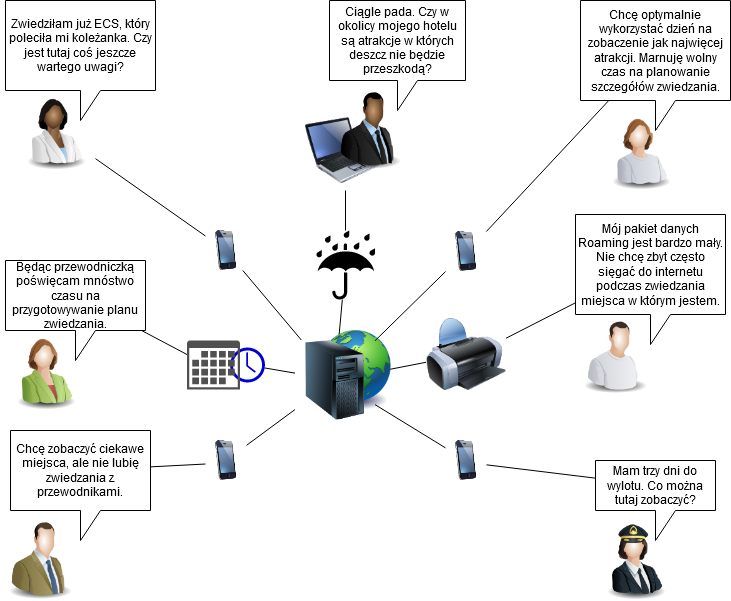
\includegraphics[width=1\textwidth]{attachments/rich-picture}
    \caption{Wzbogacony wizerunek planeru miejskiego}
    \label{fig:rich-picture}
\end{figure}

\section{Cele projektu}
\label{sec:cele-projektu}

TODO

%%! Author = Mateusz Budzisz
%! Date = 04/11/2023

\chapter{Decyzje projektowe}
\label{ch:decyzje-projektowe}

\section{Narzędzia i technologie}
\label{sec:narzedzia-i-technologie}

\subsection{Języki programowania i biblioteki}
\label{subsec:jezyki-programowania-i-biblioteki}

\subsubsection{Oprogramowanie po stronie użytkownika}
Jednym z celi projektu jest stworzenie aplikacji progresywnej dostępnej na większości urządzeń codziennego użytku tj.: komputery i smartfony.
Według statystyk prowadzonych przez Google za znaczną część konsumenckiego ruchu internetowego odpowiadają te systemy operacyjne: Android, ios, MacOS, Windows, Linux.
To aż 5 bardzo różniących się od siebie środowisk docelowych, każde z nich posiada swój dedykowany sposób wytwarzania i utrzymywania oprogramowania.
Nasz zespół składający się z czterech pracujących na etacie studentów nie byłby w stanie stworzyć a co dopiero utrzymywać rozwiązania na tylu różnych platformach na raz.
Istnieją rozwiązania niwelujące ten problem w znacznym stopniu, zespół projektowy przeanalizował część z nich pod kątem naszego doświadczenia.

\paragraph{Flutter}
Jest otwartoźródłowy zestaw narzędzi dla programistów przeznaczony do tworzenia natywnych, wieloplatformowych aplikacji mobilnych, komputerowych oraz internetowych, stworzony przez firmę Google.
Aplikacja stworzona w tej technologii pozwala na napisanie kodu źródłowego w jednej wersji i uruchomienie go na szerokiej gamie zróżnicowanych urządzeń docelowych.
Problemem tej technologii jest dość niszowy język programowania, z którym nikt z nas nie miał do czynienia oraz relatywnie słaba wydajność dostarczonego oprogramowania.

\paragraph{Electron}
Jest to otwartoźródłowy projekt, który umożliwia stworzenie oprogramowania w formie strony internetowej oraz osadzenia jej w minimalistycznej wersji przeglądarki wysyłanej wraz z aplikacją.
Dużym plusem tej technologii jest to, że na uczelni mieliśmy zajęcia z React-a, który jest jedną z opcji pisania aplikacji w Electron-ie.
Minusem tego rozwiązania jest bardzo duży rozmiar docelowej aplikacji z uwagi na potrzebę doczepienia przeglądarki internetowej poza samą aplikacją.

\paragraph{Progresywna Aplikacja Internetowa}
Z języka angielskiego Progressive Web App to aplikacja internetowa uruchamiana tak jak zwykła strona internetowa, ale umożliwiająca stworzenie wrażenia działania jak natywna aplikacja mobilna lub aplikacja desktopowa.
Technologia bardzo podobna do Electron-a, z tym że zamiast wysyłać spreparowaną przeglądarkę, polegamy na przeglądarce uprzednio zainstalowanej u użytkownika.
Plusem jest bardzo mały rozmiar docelowej aplikacji oraz relatywnie dobra wydajność, ponieważ przeglądarki internetowe są specjalnie optymalizowane pod wiele platform docelowych.
Minusem tego rozwiązania jest poleganie na przeglądarce użytkownika docelowego, która może nie wspierać wszystkich funkcjonalności.

\paragraph{Wybór}
Każda z wymienionych opcji ma swoje poważne wady.
Nasz zespół podejmując dedycję, kierował się następującymi priorytetami: znajomość technologii wewnątrz zespołu, wydajność rozwiązania.
Biorąc pod uwagę te 2 czynniki, postawiliśmy na \acrshort{pwa}\@.
Pragnąc wykorzystać komercyjne doświadczenie zespołu, zamiast używać poznanego na uczelni React-a, zaimplementujemy aplikację we framework-u Angular.

\subsubsection{Oprogramowanie niewidoczne dla użytkownika}
Nasz projekt zakłada stworzenie zaawansowanego algorytmu ustalania optymalnej trasy zwiedzania na podstawie danych czasu rzeczywistego.
Ciągłe aktualizacje danych po stronie użytkowników spowodowałoby wysokie zużycie internetu oraz ogromne obciążenie po stronie dostawców danych.
Dlatego postanowiliśmy stworzyć serwis, który będzie odpowiadać za aktualność danych oraz wyznaczanie trasy.
Z uwagi na \acrshort{pwa}, język, w którym stworzymy ten serwis, musi mieć bardzo dobre wsparcie dla protokołu HTTP\@.
Na uczelni poznaliśmy 2 technologie tworzenia takich serwisów.

\paragraph{Java}
Java to język paradygmatu obiektowego, bardzo popularny w systemach bankowych.
W trakcie zajęć na uczelni poznaliśmy sposób tworzenia serwisów \acrshort{http} w technologii Spring.
Części naszego zespołu nie podobają się konwencje narzucone przez tę technologię, jak i sposób komunikacji z bazą danych.
Należy zaznaczyć, że nikt z naszego zespołu nie posada komercyjnego doświadczenia z tą technologią.

\paragraph{.NET}
C\# to jeden z języków z rodziny .NET, który mielimy szanse poznać na uczelni.
Łączy on w sobie paradygmaty obiektowe i funkcyjne, dzięki czemu jest bardziej elastyczny, jeśli chodzi o styl programowania.
Trzy z czterech osób w naszym zespole ma doświadczenie komercyjne w tej technologi.

\paragraph{Wybór}
Z uwagi na doświadczenie zespołu postawiliśmy na C\#.

\subsubsection{Baza danych}
Na uczelni dogłębnie poznaliśmy bazę danych PostgreSql, zespół ma komercyjne doświadczenie z tą bazą, więc nie braliśmy innych rozwiązań pod uwagę.

\subsection{Narzędzia programistyczne}
\label{subsec:narzedzia-programistyczne}
Nasz zespół składa się z osób, które mają znaczne doświadczenie w oprogramowaniu, którego używa na co dzień w pracy.
Wybrany przez nas stos technologiczny składa się z .NET C\#, Angular oraz PostgreSql.
Wszystkie te technologie, pomimo iż są utrzymywane przez ogromne korporacje, są otwarto-źródłowe, co w praktyce pozwala na tworzenie narzędzi deweloperskich przez niezależnych twórców, dzięki czemu nie bylibyśmy uwiązani do konkretnego rozwiązania.
Wybór oprogramowania do tworzenia kodu został podyktowany wybraną technologią a w drugiej kolejności z uwagi na zróżnicowany sprzęt komputerowy, którym dysponujemy  dostępnością oprogramowania na wielu platformach (tj.: Windows, MacOS, Linux).

\subsubsection{.NET/C\#}
.NET to framework stworzony i rozwijany przez Microsoft wspólnie ze społecznością otwartego oprogramowania.
Pierwszym oprogramowaniem, które przychodzi nam do głowy, gdy słyszymy .NET, jest Microsoft Visual Studio.
Oprogramowanie to powstało w 1997 roku i przez wiele lat było konsekwentnie ulepszane.
W 2016 roku VS zostało wydane na komputery Mac, jednakże, po 7 latach, w 2023 roku Microsoft ogłosił zakończenie wsparcia dla wersji MacOS.
Jeśli chodzi o systemy Linux, to VS nigdy nie zostało wydane na ten system.

Zespół projektowy bardzo nie chciał uzależnić pracy nad projektem od systemu Windows, Microsoft poleca użycie programu Visual Studio Code, który jest wspierany na wszystkich systemach operacyjnych, których używamy.
Niestety VSC jest edytorem przeznaczenia ogólnego, co za tym idzie, znaczna większość specjalistycznych dla danej technologii narzędzi jest obsługiwana przy pomocy rozszerzeń.
Rozszerzenia mogą tworzyć wszyscy, jest ich całkiem sporo niestety wszystkie rozszerzenia skupiające się na technologii .NET/C\# są we wczesnej fazie rozwoju i nie wspierają tak podstawowych rzeczy, jak debugowanie kodu.
Nawet gdy dane rozszerzenie wspiera jakąś zaawansowaną funkcjonalność, to przeważnie konfiguracja takiego rozszerzenia bardzo różni się pomiędzy systemami operacyjnymi co, de facto niweczy sens wieloplatformowości.

W 2016 roku został ogłoszony JetBrains Rider niejako odpowiedź na VS na MacOS od Microsoftu.
Rider bardzo dynamicznie się rozwijał, nadganiając, a nawet prześcigając VS pod względem funkcjonalności, do momentu, w wyniku czego duża część środowiska programistycznego zaczęła go używać jako głównego narzędzia do pracy.
Programy firmy JetBrains są znane ze świetnej integracji wieloplatformowej oraz dbania o szczegóły, co zapewnia dobre doświadczenie deweloperskie.

Dzięki PJATK nasz zespół mógł przetestować, każdy z tych programów w ramach licencji edukacyjnej.
Nasze testy doprowadziły nas do decyzji, aby postawić na Ridera od JetBrains-ów, z zachowaniem możliwości uruchomienia projektu w Visual Studio, aby koledzy z dużym doświadczeniem komercyjnym opartym o VS nie musieli zmieniać swoich przyzwyczajeń.

\subsubsection{Angular}
Angular z natury bycia technologią tworzenia stron internetowych nie posiada dedykowanego środowiska programistycznego stworzonego przez jedną firmę.
Zespół tworzący ten framework stworzył własny program wspomagania deweloperów na podstawie protokółu \acrshort{lsp}, co sprowadza się do tego, że każde środowisko programistyczne wspierające ten protokół zapewni ten sam poziom wsparcia dla Angular'a.

Warto tu wyróżnić Visual Studio Code, ponieważ jest to środowisko zalecane przez twórców Angular-a, a nowe projekty tworzone w tej technologii zawierają niezbędną konfigurację potrzebną do pełnego wsparcia dla Angulara.

JetBrains też ma w swojej ofercie program do tworzenia w technologiach internetowych o nazwie WebStorm, który posiada automatyczną konfigurację dla Angular-a, jak i wielu innych technologii, więc nie potrzebuje bezpośredniego wsparcia od autorów technologi.

Mając na uwadzę fakt, że Visual Studio Code domyślnie ma skróty klawiszowe nieprzypominające innych popularnych środowisk programistycznych, których trzeba by było się nauczyć, oraz fakt, że już wybrany Rider jest niemalże identyczny w obsłudze do WebStorm'a, postawiliśmy na WebStorm'a, znowu z możliwością uruchomienia projektu w dowolnym innym środowisku, gdy ktoś będzie tego z jakiegoś powodu potrzebował.

\subsubsection{PostgreSql}
W przypadku baz danych przeważnie jest tak, że twórcy bazy danych, równocześnie do samej bazy danych rozwijają narzędzie pozwalające na administrację tą bazą.
W przypadku PostgreSql narzędzie to nazywa się pgAdmin, umożliwia kompleksową konfigurację bazy danych i administrowanie nią.

Należy jednak wspomnieć tu o integracji Ridera z bazą danych we współpracy z programem DataGrip.
Gdy mamy licencję na DataGrip-a, to wewnątrz Rider-a możemy podłączyć się do bazy danych i otrzymywać dodatkowe wsparcie w kontekście bazy danych.
Wsparcie nie ogranicza się tylko do dodatkowego kolorowania składni w zależności od dialektu wybranej bazy danych, a deweloper jest wspierany przez podpowiadanie nazw kolumn, tabeli oraz poprawność zapytań do bazy jest  weryfikowana w czasie rzeczywistym, a w przypadku wątpliwości Rider pozwala na szczegółową analizę kwerendy w DataGrip'e.

Mając na uwadze powyższe, zespół projektowy zaleca użycie DataGrip-a jako narzędzia do projektowania rozwiązań dookoła bazy danych z uwagi na kompleksową integrację z Riderem.

\subsubsection{Dalekosiężność wyborów}
W przypadku, w którym zespół zdecydowałby się na dalsze utrzymywanie bądź rozwój projektu, należy brać pod uwagę koszta oprogramowania.

Visual Studio jest najdroższym z wymienionych rozwiązań, do tego wspiera tylko wąski fragment stosu technologicznego.

Oprogramowanie JetBrains, na które postawiliśmy, jest dostępne jako poszczególne programy w formie abonamentu, jednakże najkorzystniej jest je kupować w pakietach łączonych.

Warto też wspomnieć o programie wsparcia open source firmy JetBrains, która to oferuje darmowe licencje do wszystkich swoich komercyjnych rozwiązań dla projektów o otwartym kodzie źródłowym, przy czym nasz projekt spełnia tę definicję.

Ponadto dzięki zachowaniu kompatybilności z alternatywnymi środowiskami deweloperskimi, jesteśmy w stanie małym nakładem pracy zmienić oprogramowanie nawet na darmowe.

\subsection{Dostawcy mocy obliczeniowej}
\label{subsec:dostawcy-mocy-obliczeniowej}
Wytworzone oprogramowanie potrzebuje serwerów, na których będzie wdrożone.
Zespół projektowy zna 2 podejścia do tego problemu.

\subsubsection{Oprogramowanie w chmurze}
Dostawcy oprogramowania w chmurze umożliwiają bardzo elastyczny system rozliczania się za moc obliczeniową.

Gdy aplikacja nie wymaga ciągłej pracy oraz w sposób deterministyczny można ustalić warunki czasowe dla aplikacji, możemy jej użyć w stylu \gls{on-demand}.
Sposób ten charakteryzuje bardzo korzystny sposób rozliczania, gdzie płacimy za faktycznie wykorzystany czas pracy maszyn oraz potencjalnie nieskończone możliwości horizontal-scallingu.

Wybór takiego rozwiązania mocno wpłynąłby na architekturę naszego rozwiązania.
Niejako wymusiłby na nas, podział projektu na niezależne od siebie moduły i z uwagi na bardzo skomplikowany \gls{refactoring} przy 4-osobowym zespole de facto scementowałby strukturę projektu.

Nasz projekt teoretycznie można podzielić na niezależne od siebie części o różnym zapotrzebowaniu na moc obliczeniową.
Pierwszym modułem musi być baza danych, w której będziemy trzymać graf możliwych połączeń między atrakcjami oraz informacje o samych atrakcjach, ten moduł musiałby być cały czas dostępny z uwagi na duży koszt wyprodukowania danych, przeważający koszt utrzymania bazy w sposób ciągły.
Drugim modułem mógłby być \gls{job} aktualizujący dane z OSM, urzędu miasta oraz atrakcji turystycznych, taki moduł mógłby uruchamiać się na przykład raz dziennie.
Trzecim modułem byłby serwis implementujący algorytm, dobierania trasy pomiędzy podanymi POI, taki serwis uruchamiałby się na zapytanie użytkownika i kończył swoją pracę wraz z podaniem optymalnie dobranej trasy.
Ostatnim modułem byłaby aplikacja \gls{frontend}-owa implementująca UI, włączana z osobna dla każdego użytkownika, gdy ten podejmie próbę wejścia na adres naszego rozwiązania.

Takie podejście w praktyce zmniejsza koszt utrzymania do kosztu utrzymywania bazy danych, ponieważ gdy zapotrzebowanie na pozostałe moduły drastycznie by zmalało, to nie będą one chodzić i czekać na ruch użytkowników.
Niestety uruchamianie programów na żądanie wiąże się ze znaczącym opóźnieniem wobec żądań użytkownika docelowego.
Gdy użytkownik postanowi skorzystać z naszej aplikacji, dostawca chmury obliczeniowej musi uruchomić co najmniej dwie maszyny, dla modułu 3 i 4, co czasami potrafi zająć kilka sekund.
Gdy dostawca chmury uruchomi odpowiednie maszyny, jeszcze nasze oprogramowanie wymaga czasu na obsłużenie żądania.
W przypadku modułu 3 musimy nawiązać połączenie z bazą danych, odczytać dane, zastosować na nich skomplikowany obliczeniowo algorytm i wysłać odpowiedź, obawiamy się, że w skrajnych przypadkach może to zająć za dużo czasu aby odpowiedź trafiła do użytkownika przed zamknięciem połączenia.
W przypadku modułu 4 możemy odroczyć oczekiwanie na odpowiedź modułu 3 i poinformować użytkownika o wydłużonym czasie oczekiwania, niemniej jednak, aby cokolwiek użytkownikowi pokazać i tak jesteśmy zmuszeni do wykonania kodu odpowiedzialnego za stworzenie \gls{ui}, według doświadczeń zespołu czas potrzebny na \gls{rendering} \gls{hello-world} pozostawia niewiele czasu do przekroczenia średniego time span nowego użytkownika (TODO: source).

Istnieją techniki pozwalające na optymalizację tych rozwiązań, aby wyeliminować przytoczone problemy.
Jednak opierają się one o jeszcze większą fragmentację aplikacji, na którą nie możemy sobie pozwolić z uwagi na liniowo rosnący czas potrzebny na konfigurację infrastruktury potrzebnej do skomunikowana wszystkich modułów w \glslink{hermetyzacja}{hermetyczny} sposób.
Infrastrukturę chmury internetowej w każdym ze znanych nam dostawców to jest: \acrshort{aws}, \acrshort{gcp}, \acrshort{azure} możemy wyklikać w przeglądarce internetowej.
Jednak usługi te znacząco się od siebie różnią.
Możemy tę manualną pracę zautomatyzować przy pomocy podejścia \gls{infra-as-code}, na przykład przy użyciu terraform.
Pomimo iż dostawcy oferują podobne rozwiązania, to różnią się one w sposobie konfiguracji, na przykład 1 usługa w \acrshort{gcp} to 3 usługi w \acrshort{aws}\@.
Terraform daje możliwość skorzystania z dodatkowej warstwy abstrakcji pozwalającej na opisanie architektury dla \acrshort{aws}, jak i zarówno \acrshort{gcp}, jednakże nie jest to pełne wsparcie i niektóre usługi po prostu nie pokrywają się pomiędzy dostawcami.
Ponadto Terraform nie wspiera takiej funkcjonalności dla Azure.

\subsubsection{Oprogramowanie on premise}
Oprogramowanie on premise możemy podzielić na bare metal i virtual.

Bare metal to takie, gdzie mamy fizyczny dostęp do maszyny i płacimy za konkretne podzespoły, mamy pełną kontrolę nad maszyną.
Virtual to oprogramowanie, w którym tak jak w przypadku bare-metal musimy sami zarządzać maszyną.
Różni się jednak tym, że płacimy za parametry podzespołów, nie za konkretne podzespoły.
Nie mamy też fizycznego dostępu do maszyny, ponieważ parametry, jakich potrzebujemy, mogą być mniej wymagające, niż fizyczna maszyna jest w stanie zapewnić, przez to właściciele takich maszyn stosują \glslink{virt}{wirtualizację}.

Bare metal ma taką zaletę, że jesteśmy pewni, że nikt poza nami na takiej maszynie nie będzie pracował.
Minusem jest mała elastyczność podzespołów (musimy wiedzieć, co będzie działać, z czym) oraz wysoki koszt początkowy.
W przypadku wirtualizacji na początku rozwoju aplikacji możemy poprosić o niewielkie parametry a wraz z rozwojem przeskalować parametry do naszych potrzeb.

Pomimo faktu, iż w przypadku \gls{on-prem} musimy sami zarządzać infrastrukturą, to jest to niezależne od dostawcy sprzętu, dzięki czemu można łatwo przenieść całą aplikację do innego dostawcy.
Biorąć pod uwagę ten fakt oraz brak możliwości napisania oprogramowania w sposób pełni agnostyczny względem konkretnych usług chmury obliczeniowej, zespół projektowy zdecydował się na on premise w wariancie virtual.

\subsubsection{Przegląd rynku}
\paragraph{Microsoft Azure Cloud}
Chmura obliczeniowa Microsoftu została nam udostępniona w ramach zajęć z konteneryzacji.
Microsoft udostępnia studentom jednorazowo 200\$ do wykorzystania na okres roku.
W ramach okresu edukacyjnego mamy do dyspozycji najsłabsze i najmniej stabilne maszyny dostępne w ofercie.
W trakcie zajęć natknęliśmy się na wiele problemów ze stabilnością i wydajnością tej chmury.
Jednorazowy roczny okres próbny w połączeniu z ograniczeniem budżetowym całkowicie deklasuje tą chmurę z powodu braku możliwości utrzymania rozwiązania w rozumieniu długoterminowym

\paragraph{Amazon Web Services}
Chmurę obliczeniową Amazon mieliśmy okazję zobaczyć na szkoleniu organizowanym przez Merapar.
W trakcie zajęć chmura nie sprawiła najmniejszych problemów, co pokrywa się z licznymi opiniami rynkowymi.
Niestety pomimo wielu darmowych progów zużycia, Amazon nie oferuje darmowego progu w przypadku usługi EC2 (\gls{on-prem} virtual).

\paragraph{Google Cloud Platform}
GCP zostało nam zaprezentowane w ramach projektu PJATK cloudelina.
Usługi w ramach GCP wydają się znacznie prostsze w konfiguracji oraz bardzo dobrze integrują się z Angular-em.
Niestety podobnie jak w przypadku Amazon-u, GCP nie oferuje darmowego progu dla maszyn wirtualnych.

\paragraph{Oracle Cloud Platform}
Oracle cloud jako jedyne nie posiada usług typowych dla architektury chmurowych.
Oracle daje bardzo hojny darmowy limit dla maszyn wirtualnych opartych o \glslink{arm}{architekturę arm} wynoszący 6 CPU, 24 GB RAM, 200 HDD i 100 Mbs ethernet.
Taki próg pozwoli nie tylko na wytworzenie oprogramowania, przeprowadzenie testów, ale nawet i obsługę średniej wielkości ruchu użytkowników.

\subsection{Przechowywanie kodu oraz potok ciągłego wdrożenia}
\label{subsec:przechowywanie-kodu-oraz-potok-ciagego-wdrozenia}

W trakcie zajęć na uczelni, jak i pracy indywidualnej członków zespołu projektowego poznaliśmy 2 systemy kontroli wersji.
Są to GIT oraz Mercurial.

GIT pod każdym względem jest lepszy od Mercurial, sam Mercurial jest uznany za projekt bez rozwoju.
Zespół projektowy postanowił oprzeć swoją pracę na podstawie GIT, natomiast nie chcemy samodzielnie zarządzać serwerem repozytorium.

\subsubsection{Usługi internetowe ułatwiające pracę wielu współbieżną w repozytorium GIT}
\paragraph{GitLab}
\paragraph{BitBucket}
\paragraph{Microsoft Azure Repositories}
\paragraph{Github}



	%! Author = Wiktor Rostkowski, Mateusz Budzisz
%! Date = 05/24/2024

\chapter{Kontekst projektu}
\label{ch:kontekst-projektu}

\section{Aspekty społeczne}
\label{sec:aspekty-spoleczne}

W erze „fake news”, gdzie występuje duża ilość niskiej jakości informacji, trudno znaleźć wiarygodne źródła informacji.
Konieczne jest wielokrotne weryfikowanie źródeł przez każdą grupę społeczną,~od~młodzieży~po~seniorów~\cite{fakenews}.

\indent Nasza aplikacja spełnia liczne potrzeby turystów pragnących efektywnie zaplanować zwiedzanie miasta wykorzystując rzetelne~i~pewne informacje~o~jego atrakcjach,~a~także~bez~znacznego nakładu czasowego.
Turystyczny planer miejski oferuje kompleksowy zbiór informacji niezbędnych~dla~każdego turysty, wolny~od~niedopowiedzeń.
Przewidywaną grupą docelową~są~osoby odwiedzające daną miejscowość, posiadające umiarkowaną znajomość technologii, które chcą dostosować podróż zarówno~dla~siebie,~jak~i~dla~większych grup,~na~przykład wycieczek~dla~znajomych.

\indent Na~potrzeby turystów proponowane jest rozwiązanie~z~następującymi funkcjami:

\begin{enumerate}
    \item Interaktywna mapa~z~naniesionymi atrakcjami turystycznymi zawierająca zawsze aktualne informacje~o~atrakcjach turystycznych.
    \item Generowanie planu wycieczki~na~podstawie wybranych miejsc oraz trasy pomiędzy nimi.
    \item Automatyczna aktualizacja planu zwiedzania~na~podstawie dynamicznych wydarzeń, takich~jak~zmiana pogody, rozkład jazdy~czy~dostępność atrakcji,~co~umożliwia planowanie~w~czasie rzeczywistym.
\end{enumerate}

Dzięki~tym~funkcjonalnościom możliwe jest uniknięcie wielogodzinnego poszukiwania informacji~na~temat dostępnych miejsc oraz efektywne zaplanowanie podróży.

\indent Przeanalizowano społeczne aspekty wdrożenia proponowanego rozwiązania,~w~wyniku czego zidentyfikowano zarówno pozytywne,~jak~i negatywne skutki.

\indent Jednym~z~założeń projektu jest wspieranie rozwoju turystyki.
Aplikacja promuje niszowe atrakcje, prezentując~na~mapie tylko wybrane miejsca.
Dzięki mniejszej liczbie znaczników, mniej popularne atrakcje mają większą szansę~na~znalezienie przez użytkowników.

\indent Przedstawione informacje~są~dostępne~dla~każdego odwiedzającego~i~obejmują~nie~tylko atrakcje turystyczne,~ale~także dostępny transport,~a~w przyszłości również zakwaterowanie~i~restauracje.
Dzięki temu podróżowanie staje~się~łatwiejsze~i~nie wymaga posiadania przewodnika,~a~samodzielna koordynacja~nie~wiąże~się~z nadmiernym obciążeniem poznawczym. \newline
Człowiek podczas zwiedzania miasta skupia~się~na doświadczaniu~i~zwiedzaniu,~a~nie selekcjonowaniu danych, informacji~i~podejmowaniu decyzji.
Aplikacja zapobiega obciążeniu poznawczemu (ang.\ cognitive load), które jest konsekwencją nadmiaru opcji dostępnych~w~danym mieście.
Dzięki "uwolnionym zasobom" możliwa jest koncentracja użytkowników~na~faktycznym poznawaniu miasta~\cite{cognitive-biases}.

\indent Dodatkowo, rezygnacja~z~przetwarzania danych wrażliwych~w~przyjętym modelu zwiększa poczucie bezpieczeństwa użytkowników.
Korzystanie~z~systemu~nie~wiąże~się~z ryzykiem utraty~lub~nieuprawnionego wykorzystania danych,~co~jest kluczowe~dla~zachowania zaufania.
Celem jaki towarzyszył zespołowi projektowemu, było zaspokajanie potrzeb użytkowników, uwzględniając~ich~interesy oraz przestrzeganie obowiązującego prawa, przy jednoczesnym zachowaniu poufności.

\indent Wytworzona aplikacja pozwala użytkownikom łatwo~i~samodzielnie uzyskać dostęp~do~trudno dostępnych informacji.
Dzięki wygodnemu planowaniu~w~formie interfejsu drag-and-drop, aplikacja zmniejsza atrakcyjność płatnych przewodników oferujących gotowe plany zwiedzania
W rezultacie może~to~generować negatywne konsekwencje społeczne~w~postaci zwiększonego poczucia zagrożenia wśród przewodników turystycznych działających~na~wolnym rynku.

\indent Warto również wspomnieć,~że~podczas implementacji aplikacji,~z~powodu braku czasu, pominięto kilka funkcji, które~w~aktualnej wersji mogą generować potencjalne niezadowolenie użytkowników.
Na przykład, brak możliwości rezerwacji terminów~w~wybranych atrakcjach może~być~problematyczny~dla~użytkowników, szczególnie~gdy~wymagana jest wcześniejsza rezerwacja.
Ponadto,~nie~zdążono dodać integracji~z~zakwaterowaniem~i~lokalami gastronomicznymi.
Niemniej jednak, aplikacja została przystosowana~dla~osób~z~wadami wzroku,~co~stanowi istotny krok~w~kierunku zwiększenia~jej~dostępności~i~inkluzywności.

\indent W~związku~z~powyższym zidentyfikowano obszary wymagające udoskonalenia proponowanego systemu,~aby~skuteczniej odpowiadał~na~potrzeby użytkowników oraz wywierał większy wpływ społeczny.
Kluczowym aspektem~z~perspektywy społecznej~w~przyszłości będą elementy sieci społecznościowej, takie~jak~recenzje atrakcji turystycznych oraz możliwość dzielenia~się~planami zwiedzania~z~innymi użytkownikami.



\pagebreak
\section{Analiza ryzyka}
\label{sec:analiza-ryzyka}

\begin{longtable}{|p{.1\linewidth}|p{.15\textwidth}|p{.2\textwidth}|p{.25\textwidth}|p{.25\textwidth}|}
    \hline
    Ryzyko & Czynniki ryzyka & Charakterystyka ryzyka & Prawdopodobieństwo wystąpienia ryzyka & Planowane działania \\
    \hline
    \multirow{6}{=}{\parbox[c]{12cm}{\rotatebox[origin=c]{90}{\multirow{6}{=}{\textbf{Nieukończenie projektu w terminie}}}}}& Rozpad grupy & Odejście jednego z członków zespołu & niskie
    & Przejrzysta komunikacja w zespole i ustalenie wersji MVP produktu, która może zostać ukończona w uszczuplonym składzie \\
    \cline{2-5}
    & Czasowa niedostępność / niedyspozycja członka zespołu & Nagła lub zaplanowana nieobecność członka zespołu & średnie
    & Możliwie wczesne sygnalizowanie planowanej nieobecności \\
    \cline{2-5}
    & Zbyt ambitne założenia projektowe & Zaplanowane prace wykraczają poza moce przerobowe członków zespołu & średnie
    & Śledzenie postępu prac pod kątem wykonalności i zmieszczenia się w ograniczeniach czasowych, konsultacja z promotorem \\
    \cline{2-5}
    & Pełzające wymagania & Ciągle powiększana pula wymagań, zwiększająca zakres prac do wykonania & średnie & Iteracyjna implementacja i dopracowywanie wymagań pod implementację \\
    \cline{2-5}
    & Nauka nowych technologii / języków programowania & Zwiększenie ilości czasu potrzebnej na ukończenie zadania &
    wysokie & Używanie technologii opanowanych przez zespół projektowy \\
    \cline{2-5}
    & Problem z komunikacją w zespole & Brak właściwego przepływu informacji między członkami zespołu & średnie
    & Cykliczne spotkania członków zespołu w celu omawiania postępu prac i planowania kolejnych działań \\
    \hline
    \pagebreak
    \hline
    \multirow{5}{=}{\parbox[c]{10cm}{\rotatebox[origin=c]{90}{\multirow{5}{=}{\textbf{Produkt nie spełnia wymagań projektowych}}}}} & Błędna analiza rynku & Niewłaściwe rozpoznanie potrzeb potencjalnych użytkowników oraz rozwiązań konkurencyjnych & niskie
    & Konsultacje z promotorem, stworzenie profilu docelowego użytkownika \\
    \cline{2-5}
    & Niespełnienie wymagań klientów & Finalny produkt nie zapewnia zakładanych korzyści dla użytkownika końcowego & średnie
    & Konsultacje z promotorem, cykliczna analiza kierunku rozwoju produktu \\
    \cline{2-5}
    & Wydanie wersji zawierającej krytyczne błędy & Produkt zawiera błędy uniemożliwiające korzystanie z jego podstawowych funkcjonalności & niskie
    & Napisanie odpowiednich testów sprawdzających działanie funkcjonalności \\
    \cline{2-5}
    & Zmiany w usługach zależnych & Wyłączenie lub zmiana warunków na jakich udostępniane są API wpływa na dostarczane funkcjonalności & średnie
    & Ustalenie alternatywnych dostawców potrzebnych usług \\
    \cline{2-5}
    & Zły dobór narzędzi projektowych & Wybrane narzędzia są nieodpowiednie do zaplanowanych prac & niskie
    & Zaznajomienie się z dokumentacją używanych narzędzi, konsultacje w zespole \\
    \hline
    \pagebreak
    \hline
    \multirow{2}{=}{\parbox[c]{3.5cm}{\rotatebox[origin=c]{90}{\multirow{2}{=}{\textbf{Niewłaściwe zaplanowanie przebiegu prac}}}}} & Przyjęcie nieodpowiedniej strategii projektowej & Przyjęta strategia nie pozwala na uzyskanie wymaganych rezultatów przy dostępnych zasobach & wysokie
    & Stałe monitorowanie kierunku prac, konsultacje z promotorem \\
    \cline{2-5}
    & Nierozpatrzenie potencjalnych przypadków brzegowych & Konieczność uwzględnienia nieprzewidzianych prac & wysokie
    & Staranne analizowanie planowanych funkcjonalności i ich wpływu na produkt \\
    \hline
    \multirow{1}{=}{\parbox[c]{3.5cm}{\rotatebox[origin=c]{90}{\multirow{1}{=}{\textbf{Zdarzenia nieprzewidziane}}}}}& Zbyt gwałtowny rozrost liczby użytkowników & Liczba użytkowników przekracza zaplanowane możliwości techniczne produktu & niskie
    & Projektowanie produktu z możliwością jego skalowania \\
    \hline

\end{longtable}
\pagebreak
\section{Rozwiązania konkurencyjne}
\label{sec:rozwiazania-konkurencyjne}
Na rynku dostępne~są~obecnie różne rozwiązania mające~na~celu ułatwienie planowania podróży~i~posiadające różny zakres funkcjonalności.
Użytkownik może napotkać rozbudowane aplikacje integrujące wiele funkcjonalności takich~jak~układanie list atrakcji~do~zwiedzania, optymalizacja tras podróży, dokumentowanie poniesionych wydatków, tworzenie list ułatwiających planowanie (listy czynności~do~wykonania, listy zakupów, listy ułatwiające organizację pakowania), synchronizacja naszych planów podróży~ze~znajomymi, integrowanie rezerwacji hotelowych~i~lotów.
Aplikacje skupiające~się~na wspomaganiu procesu zwiedzania sugerują użytkownikowi interesujące punkty~w~jego lokalizacji (interesujące miejsca, hotele, restauracje, sklepy itp.)~i~oznaczają~je~na mapie.
Dodatkowo bardzo często~są~wyposażone~w~rozbudowany opis danej atrakcji, czasem również~w~formie głosowej,~co~umożliwia zamienienie urządzenia mobilnego~w~osobisty audio przewodnik.
Kolejną funkcjonalność stanowi możliwość dokonywania zakupu biletów~i~rezerwowania atrakcji bezpośrednio~z~poziomu aplikacji turystycznej.
Poniżej przedstawiono przykłady najpopularniejszych obecnie rozwiązań ułatwiających planowanie zwiedzania.

\subsection{Wanderlog}
\label{subsec:wanderlog}
Jest~to~aplikacja reklamująca~się~jako planer podróży,~ze~szczególnym naciskiem~na~organizowanie wakacji oraz wycieczek samochodem.
W wersji podstawowej jest darmowa, posiada również płatną wersję premium  oferującą dodatkowe funkcjonalności.
Aplikacja jest dostępna poprzez przeglądarkę internetową~jak~również poprzez dedykowaną aplikację~na~urządzenia mobilne.
Wanderlog umożliwia układanie list~z~interesującymi użytkownika miejscami~i~wydarzeniami, które~są~graficznie przedstawione~w~postaci pinezek~na~mapie google.
Po wybraniu lokalizacji~i~daty podróży, użytkownik może dokonać przeglądu ofert noclegów.
Aplikacja umożliwia tworzenie planów podróży razem~z~innymi użytkownikami oraz~ich~synchronizację~w~czasie rzeczywistym.
Ponadto użytkownik~ma~dostęp~do~spersonalizowanych sugestii.

\subsection{TripIt}
\label{subsec:tripit}
Jest~to~planer podróży integrujący wiele funkcjonalności~w~celu maksymalnego ułatwienia użytkownikowi procesu podróżowania.
Stanowi alternatywę~dla~wspomnianej wcześniej aplikacji Wanderlog~i~również posiada darmową wersję podstawową oraz wersję płatną opartą~na~modelu subskrypcyjnym, która posiada dodatkowe funkcjonalności.
W wersji podstawowej użytkownik~ma~możliwość układania planów podróży, które~są~dostępne~na~wielu urządzeniach jednocześnie.
Udostępnia statystyki, wytyczne dotyczące restrykcji COVID-19 oraz umożliwia dodawanie zdjęć, kodów~QR~oraz plików~PDF~do planów podróży.
Aplikacja zapewnia nawigację między punktami, mapy lotnisk, sugestie~co~do interesujących miejsc blisko lokalizacji użytkownika,~jak~również informowania~o~poziomie niebezpieczeństwa danej okolicy.
Podstawowa wersja aplikacji umożliwia również dzielenie~się~planami~z~innymi użytkownikami oraz synchronizację kalendarza.
W wersji płatnej użytkownik~ma~dostęp~do~szeregu funkcjonalności ułatwiających podróżowanie samolotem, np.~informacja~o~dostępności lepszych miejsc, przypomnienia~o~zarezerwowanych lotach, powiadomienia~o~statusie lotów~w~czasie rzeczywistym, mapy lotnisk wraz~ze~szczegółowymi informacjami~o~położeniu obiektów, informacje~o~punkcie odbioru bagażu.

\subsection{Harmony}
\label{subsec:harmony}
Umożliwia tworzenie planów podróży wraz~ze~znajomymi~w~czasie rzeczywistym oraz synchronizację~z~kalendarzem Google.
Ponadto aplikacja umożliwia śledzenie poniesionych wydatków~i~podziału kosztów~na~poszczególne osoby.
Użytkownik~ma~możliwość otrzymywania sugestii generowanych przez~AI~dotyczących interesujących miejsc~w~danej lokalizacji,~jak~również rezerwowania wycieczek~w~aplikacji.
Aplikacja umożliwia również tworzenie list rzeczy~do~wykonania~w~celu łatwego śledzenia postępów.
Obiekty~do~zwiedzania~są~zwizualizowane~na~mapie Google~w~postaci pinezek.

\subsection{Rove.me}
\label{subsec:rove.me}
Jest~to~aplikacja, która sugeruje użytkownikowi najlepszy czas~na~odwiedzenie danego miejsca~lub~wydarzenia~w~ciągu roku.
Aplikacja informuje również~o~typowej pogodzie występującej~w~interesującym użytkownika miejscu~z~uwzględnieniem pory roku~lub~daty.

\subsection{Roadtrippers}
\label{subsec:roadtrippers}
Umożliwia tworzenie planów podróży~ze~szczególnym uwzględnieniem podróży samochodem.
Poprawione zdania z uwzględnieniem "aplikacja":

Użytkownik oznacza~na~mapie interesujące~go~miejsca, takie jak atrakcje, hotele, stacje paliw, sklepy itp.
Aplikacja udostępnia informacje~o~odległości~od~celu podróży~i~szacowanym czasie dotarcia~do~niego.
Aplikacja skierowana jest~do~użytku~na~terenie Stanów Zjednoczonych.

\subsection{Visit a City}
\label{subsec:visit-a-city}
Użytkownik~ma~możliwość tworzenia list obiektów~do~zwiedzania,~jak~również rezerwowania wycieczek~i~aktywności~w~oparciu~o~dużą bazę dostępnych lokalizacji.
Posiadają~one~rozbudowane informacje~i~oceny dodawane przez innych użytkowników,~na~podstawie których możliwe jest dokonywanie wyborów, ponadto aplikacja sugeruje interesujące miejsca~w~pobliżu lokalizacji użytkownika.
Aplikacja jest dostępna mobilnie~na~urządzeniach~z~systemem~iOS~i Android.

\subsection{SmartGuide}
\label{subsec:smartguide}
Zamysłem aplikacji jest dostarczenie użytkownikom platformy dzięki, której urządzenie osobiste może zostać zamienione~w~przewodnik turystyczny.
Zwiedzanie odbywa~się~po zaplanowanych trasach,~a~dzięki śledzeniu lokalizacji użytkownika~za~pomocą nawigacji GPS, aplikacja może określić, kiedy osoba zwiedzająca dotarła~do~interesującego punktu~i~odtworzyć zapis audio~z~opisem obiektu.
Informacje~o~oglądanym obiekcie dostępne~są~również~w~formie tekstowej.
Aplikacja skierowana jest~nie~tylko~do~turystów,~ale~również~do~organizatorów wycieczek, którzy mogą tworzyć własne trasy zwiedzania.

\subsection{Fodor's City Guide}
\label{subsec:fodor's-city-guide}
Aplikacja rekomenduje użytkownikowi najciekawsze miejsca~do~zwiedzania oraz najlepsze restauracje, hotele~i~sklepy,~jak~również umożliwia rezerwację tych usług jest dostępna jest~na~urządzeniach~z~systemem iOS\@.

\subsection{Tripadvisor}
\label{subsec:tripadvisor}
Aplikacja umożliwia planowanie wycieczek, rezerwację usług ~w~oparciu między innymi~o~rekomendacje, opinie oraz wskazówki innych użytkowników.
Rekomendowane miejsca znajdujące~się~w~pobliżu lokalizacji użytkownika~są~przedstawione~na~mapie~w~formie pinezek.
Aplikacja umożliwia również dostęp~do~zakupionych biletów~w~formie elektronicznej.
Jest dostępna~na~urządzeniach~z~systemem~iOS~i~Android.

\subsection{Podsumowanie}
\label{subsec:podsumowanie}
W tabeli poniżej przedstawiono szczegółowe porównanie wszystkich konkurencyjnych rozwiązań, uwzględniając ich główne funkcje.

\newgeometry{top=0.5cm,bottom=0.5cm,left=2.7cm,right=0.5cm}
\begin{landscape}

    \begin{longtable}{|>{\raggedright\arraybackslash}p{5cm}|>{\centering\arraybackslash}p{1.5cm}|>{\centering\arraybackslash}p{1.5cm}|>{\centering\arraybackslash}p{1.5cm}|>{\centering\arraybackslash}p{1.5cm}|>{\centering\arraybackslash}p{1.5cm}|>{\centering\arraybackslash}p{1.5cm}|>{\centering\arraybackslash}p{1.5cm}|>{\centering\arraybackslash}p{1.5cm}|>{\centering\arraybackslash}p{1.5cm}|}
        \hline
        \textbf{Funkcjonalności} & \textbf{Wanderlog} & \textbf{TripIt} & \textbf{Harmony} & \textbf{Rove.me} & \textbf{Roadtrippers} & \textbf{Visit a City} & \textbf{SmartGuide} & \textbf{Fodor’s City Guide} & \textbf{Tripadvisor} \\
        \hline
        Układanie list atrakcji & Tak & Tak & Tak & Nie & Tak & Tak & Nie & Tak & Tak \\
        \hline
        Optymalizacja tras podróży & Tak & Tak & Nie & Nie & Tak & Nie & Tak & Nie & Nie \\
        \hline
        Dokumentowanie wydatków & Nie & Tak & Tak & Nie & Nie & Nie & Nie & Nie & Nie \\
        \hline
        Tworzenie list czynności & Tak & Tak & Tak & Nie & Nie & Nie & Nie & Nie & Nie \\
        \hline
        Synchronizacja planów z innymi użytkownikami & Tak & Tak & Tak & Nie & Nie & Nie & Nie & Nie & Tak \\
        \hline
        Rezerwacje hotelowe i lotów & Tak & Tak & Tak & Nie & Nie & Tak & Nie & Tak & Tak \\
        \hline
        Sugestie interesujących miejsc & Tak & Tak & Tak & Tak & Nie & Tak & Tak & Tak & Tak \\
        \hline
        Informacje turystyczne (tekstowe) & Tak & Tak & Tak & Tak & Tak & Tak & Tak & Tak & Tak \\
        \hline
        Informacje turystyczne (audio) & Nie & Nie & Nie & Nie & Nie & Nie & Tak & Nie & Nie \\
        \hline
        Zakup biletów i rezerwacja atrakcji & Nie & Tak & Tak & Nie & Nie & Tak & Nie & Tak & Tak \\
        \hline
        Mapy lotnisk, nawigacja między punktami & Nie & Tak & Nie & Nie & Nie & Nie & Nie & Nie & Nie \\
        \hline
        Informacje o restrykcjach COVID-19 & Nie & Tak & Nie & Nie & Nie & Nie & Nie & Nie & Nie \\
        \hline
        Informacje o pogodzie & Nie & Nie & Nie & Tak & Nie & Nie & Nie & Nie & Nie \\
        \hline
        Synchronizacja z kalendarzem & Nie & Tak & Tak & Nie & Nie & Nie & Nie & Nie & Nie \\
        \hline
        Sugestie dotyczące czasu wizyty & Nie & Nie & Nie & Tak & Nie & Nie & Nie & Nie & Nie \\
        \hline
        Powiadomienia o statusie lotów & Nie & Tak (wersja płatna) & Nie & Nie & Nie & Nie & Nie & Nie & Nie \\
        \hline
        Oznaczenie obiektów na mapie & Tak & Tak & Tak & Nie & Tak & Tak & Tak & Tak & Tak \\
        \hline
        Wersja mobilna (iOS, Android) & Tak & Tak & Tak & Tak & Tak & Tak & Tak & Tak & Tak \\
        \hline
    \end{longtable}

\end{landscape}
\restoregeometry

Wymienione aplikacje różnią się poziomem rozbudowania i co za tym idzie oferowanymi funkcjonalnościami.
Wspólnym mianownikiem jest możliwość tworzenia list z obiektami do odwiedzenia.
Najbardziej rozbudowane aplikacje umożliwiają rezerwowanie usług oraz środków transportu, a także ustalanie optymalnych tras podróży.
Każda z aplikacji oferuje graficzne oznaczenie obiektów na mapie.
Aplikacje pełniące funkcję przewodników wyposażone są w informacje turystyczne na temat obiektów odwiedzanych przez użytkownika, czasami również w formie audio.
Użytkownik może również kierować się opiniami i wskazówkami innych zwiedzających, które zostały przez nich zamieszczone na temat danego obiektu, czy usługi.
Na ten moment wydaje się jednak, że żadna z aplikacji nie dysponuje możliwością dynamicznego i zautomatyzowanego układania planu zwiedzania, który jest dostosowany do zainteresowań i możliwości czasowych użytkownika odwiedzającego dane miejsce.

\section{Aspekty biznesowe}
\label{sec:aspekty-biznesowe}
\subsection{Przegląd rynku}
\label{sec:przeglad-rynku}
Założeniem zespołu projektowego było stworzenie produktu unikalnego na skalę światową, aby wprowadzić nowatorskie rozwiązanie na rynek polski oraz międzynarodowy. W związku z tym przeprowadziliśmy analizę konkurencyjnych rozwiązań. Po przeszukaniu istniejącego oprogramowania doszliśmy do wniosku, że nikt wcześniej nie stworzył podobnego produktu.
Nasze rozwiązanie umożliwia użytkownikowi dynamiczne dostosowanie planu podróży na podstawie aktualnej pogody, zgodnie z jego dostępnością czasową w przystępny sposób. Dodatkowo użytkownik zawsze ma dostęp do informacji o dostępności wybranych atrakcji.
\subsection{Model biznesowy}
\label{sec:aspekty-biznesowy}
Projekt został początkowo stworzony jako część pracy dyplomowej. Jednakże jego potencjał i unikalne rozwiązania sprawiają, że może zostać z powodzeniem skomercjalizowany.
Do dokładnej analizy możliwości komercjalizacji naszego projektu wykorzystaliśmy Business Model Canvas opracowanego przez Alexander Osterwalder  utworzonego na podstawie \cite{bmc}.
Poniżej przedstawiono kierunki oraz możliwości komercjalizacji projektu, w operciu o poszczególne elementy szablonu.
\begin{enumerate}[label=\Roman*.]
    \item problem (potrzeby klientów):
    \begin{enumerate}[label=\alph*.]
        \item planowanie wycieczki zajmuje dużo czasu;
        \item nie ma jednego zbioru wszystkich atrakcji;
        \item trzeba kordynować dużo informacji:
        \begin{enumerate}[label=\roman*.]
            \item podane aktualne warunki pogodowe oraz rekomendacje do zwiedzania;
            \item czas otwarcia atrakcji;
            \item dojście do atrakcji;
            \item możliwość dodania przerwy w zwiedzaniu;
            \item proponowany czas zwiedzania;
        \end{enumerate}
        \item trudne utworzenie wycieczki we własnym zakresie na ostatnią chwilę;
        \item potrzeba informacji w jednym miejscu;
    \end{enumerate}
    \item segmentacja klientów(grupy klientów z tymi problemami):
    \begin{enumerate}[label=\alph*.]
        \item geograficzne:
        \begin{enumerate}[label=\roman*.]
            \item osoba posługująca się językiem polskim;
            \item osoba posługująca się językiem angielskim;
        \end{enumerate}
        \item demograficznie brak ograniczeń;
        \item zachowawcze:
        \begin{enumerate}[label=\roman*.]
            \item klienci preferujący bezpieczeństwo i niezawodność;
            \item klienci unikalni, którzy unikają ryzyka;
            \item osoba szukająca oszczedności czasu lub nie mająca wiele czasu;
            \item klienci ceniący tradycję i sprawdzone rozwiązania;
        \end{enumerate}
        \item psychologiczne:
        \begin{enumerate}[label=\roman*.]
            \item prowadzące aktywny styl życia(np. podróżniczy);
            \item osobowość: ciekawość świata, otwartość;
            \item otwarte na nowe doświadczenia;
        \end{enumerate}
    \end{enumerate}
    \item marketingowe kanały komunikacji:
    \begin{enumerate}[label=\roman*.]
        \item przeglądarka google;
        \item przeglądarka bing;
        \item najmu okazjonalnego do promowania poprzez broszurę informacyjną o naszej aplikacj;
        \item strona urzędu miasta;
        \item informacja turystyczna;
    \end{enumerate}
    \item relacje z klientami:
    \begin{enumerate}[label=\roman*.]
        \item fanpage aplikacji;
        \item google ads;
        \item newsletter;
    \end{enumerate}
    \item propozycja wartości naszego rozwiązania:
    \begin{enumerate}[label=\alph*.]
        \item nowość (innowacyjne rozwiązania dla konkurencji):
        \begin{enumerate}[label=\roman*.]
            \item istniejące rozwiązania oferują tylko część funkcjonalności związanych z planowaniem zwiedzania, nasza aplikacja to kompleksowe rozwiązanie;
            \item zbiór atrakcji z informacjami od godzin użytkowania po informacje jak rejestrować/kupować bilety w jednej konsekwentnej stronie internetowej;
            \item automatyczne generowanie trasy;
        \end{enumerate}
        \item dostosowanie do klienta(sposoby rozwiązań dedykowanych dla typów klientów):
        \begin{enumerate}[label=\roman*.]
            \item obrazowo pokazana usługa punkt po punkcie (klient wzrokowiec);
            \item strona z listownie przedstawionymi \glslink{poidef}{POI} (klient techniczny);
            \item interfejs graficzny przystosowany dla osób z dysfunkcjami wzroku;
        \end{enumerate}
        \item wykonanie (korzyści z zadania):
        \begin{enumerate}[label=\roman*.]
            \item wartość w formie realizacji celu zaplanowania podróży i jej rozłożenia w czasie;
            \item prosta mapa z wszystkimi punktami zainteresowań \glslink{poidef}{POI};
            \item możliwość zapisywania ulubionych punktów;
            \item plan podróży automatycznie uaktualnia się względem aktualnie  czasu;
        \end{enumerate}
        \item cena:
        \begin{enumerate}[label=\roman*.]
            \item tylko lokalny przewodnik może dostarczyć takie informacje w tak krótkim czasie;
            \item redukcja kosztów czasowych stworzenia odpowiedniego planu podróży;
        \end{enumerate}
        \item dostępność (nowy produkt bez ograniczeń):
        \begin{enumerate}[label=\roman*.]
            \item aplikacja agreguje funkcjonalność istniejących aplikacji. Dzięki temu można traktować ją jako nowość;
        \end{enumerate}
        \item wygoda oraz użyteczność (nowe możliwości):
        \begin{enumerate}[label=\roman*.]
            \item aplikacja umożliwia tworzenie planów zwiedzania, bez konieczności znania takich miejsc. Wystarczy wybrać je z mapy lub z listy;
            \item aplikacja automatyzuje trasy zwiedzania;
            \item aplikacja daje możliwość łatwego w dostępie kalendarza;
        \end{enumerate}
        \item zmniejszenie ryzyka (ułatwienia dla użytkowników):
        \begin{enumerate}[label=\roman*.]
            \item aplikacja podaje dokładne wskazanie wejścia do danego \glslink{poidef}{POI};
            \item informacje o wymaganej rezerwacji do danego \glslink{poidef}{POI};
            \item aktualne informacje o godzinach otwarcia, rekomendowane informacje o pogodzie dla \glslink{poidef}{POI};
            \item wskazanie o czasach otwarcia kas biletowych  \glslink{poidef}{POI};
        \end{enumerate}
    \end{enumerate}
    \item zakładane kluczowe zasoby:
    \begin{enumerate}[label=\alph*.]
        \item zasoby materialne (potrzebne nakłady materiale potrzebne do komercjalizacji):
        \begin{enumerate}[label=\roman*.]
            \item infrastruktura chmurowa Oracle;
            \item licencja na bibliotekę Entity Framework Extensions;
            \item licencja na kafelki mapy \glslink{stadiamaps}{Stadia Maps};
            \item licencja na środowiska deweloperskie;
            \item domena internetowa;
        \end{enumerate}
        \item zasoby intelektualne (aktualnie posiadane o zrealizowania projektu):
        \begin{enumerate}[label=\roman*.]
            \item wiedza autorów na temat działania projekt;
            \item prawa intelektualne do pracy inżynierskiej;
            \item baza danych \glslink{osm}{open street map};
            \item baza danych komunikacji miejskiej;
            \item baza danych pogodowych;
            \item baza danych noclegowni;
            \item baza danych lokali gastronomicznych;
        \end{enumerate}
        \item zasoby ludzkie (dostępne):
        \begin{enumerate}[label=\roman*.]
            \item \sout{pierwotnie czteroosobowy zespół projektowy} został dwuosobowy zespół projektowy;
        \end{enumerate}
        \item zasoby finansowe (potrzebne):
        \begin{enumerate}[label=\roman*.]
            \item finansowanie infrastruktury serwerowej;
            \item zakup i odnowienie domeny;
        \end{enumerate}
    \end{enumerate}
    \item aktywności ważne dla utrzymania relacji z klientami:
    \begin{enumerate}[label=\alph*.]
        \item bezawaryjność działającej aplikacji;
        \item aktualne dane;
        \item szybkość realizacji działąnia
    \end{enumerate}
    \item przychody:
    \begin{enumerate}[label=\alph*.]
        \item nieinwazyjne reklamy w aplikacji;
        \item sprzedaż umieszczenia punktów na mapie:
        \begin{enumerate}[label=\roman*.]
            \item restauracje;
            \item noclegownie;
            \item prywatne usługi związane z turystyką;
        \end{enumerate}
        \item leasing sprzedaż aplikacji poprzez dostosowanie aplikacji pod konkretne miasto na zamówienie;
        \item usługa abonamentowa np. wariant, przy zwiększonej ilości użytkowników darmowy użytkownik ma ograniczoną ilość zapytań (np. 30 na dzień);
        \item opłata maklerska możliwość rozwoju o sprzedaż biletów (komunikacja / atrakcje) jako pośrednik;
    \end{enumerate}
    \item koszty związane z projektem:
    \begin{enumerate}[label=\alph*.]
        \item koszta stałe:
        \begin{enumerate}[label=\roman*.]
            \item infrastruktura chmurowa: 150\$ / miesięcznie;
            \item licencja JetBrains 65 * 2€ / miesięcznie;
            \item licencja StadiaMaps 250\$ / miesięcznie;
            \item licencja OpenMeteo 29€ / miesięcznie;
            \item pensja dla pracowników;
        \end{enumerate}
        \item koszta zmienne:
        \begin{enumerate}[label=\roman*.]
        \item dostosowanie aplikacji pod miasto (finansowane przez miasto);
        \item marketing (Google Ads);
        \end{enumerate}
    \end{enumerate}
    \item kluczowe partnerstwo (bez tego typu partnerów nasza aplikacja nie mogłaby spełniać swoich założeń):
    \begin{enumerate}[label=\alph*.]
        \item krytyczni partnerzy:
        \begin{enumerate}[label=\roman*.]
            \item \glslink{osm}{OpenStreetMap}:  aktualizacja mapy miejskiej, partnerstwo na zasadzie dobrowolnej dotacji dla wolontariuszy nanoszących poprawki na mapę;
        \end{enumerate}
        \item normalni partnerzy (można zastąpić innym rozwiązaniem):
        \begin{enumerate}[label=\roman*.]
            \item \glslink{stadiamaps}{Stadia Maps};
            \item \glslink{openmeteo}{OpenMeteo};
            \item Overpass API;
            \item OpenAI Chat GPT: Analiza stron internetowych w celu ekstrakcji danych;
        \end{enumerate}
    \end{enumerate}
\end{enumerate}
\subsection{Propozycja realizacji komercjalizacji}
\label{sec:propozycja-komercjalizacji}
\indent Do zrealizowania potencjału projektu komercyjnie potrzebna jest persona, która:
\begin{enumerate}[label=\roman*.]
    \item jest właścicielem firmy;
    \item chce posiadać lub posiada markę powiązaną z turystyką;
    \item posiada zespół marketingowy lub posiada budżet na taki zespół;
    \item posiada aspiracje na produkt miedzynarodowy;
\end{enumerate}
\indent Działania, które można zrealizować, aby prezentowany system mógł sprostać oczekiwaniom komercjalizacji:
\begin{enumerate}[label=\roman*.]
    \item zmodyfikować widok atrakcji z miejscem na baner z reklamą;
    \item zmodyfikować widok kalendarza z miejscem na baner z reklamą;
    \item podpisać umowy marketingowe z gastronomią;
    \item podpisać umowy marketingowe z noclegowniami oraz hotelami;
    \item podpisać umowy pośrednika do sprzedaży biletów z atrakcjami;
    \item szukanie miast chętnych wzięcie w leasing aplikacji dedykowanej na miasto;
\end{enumerate}

	%! Author = Wiktor Rostkowski
%! Date = 29/04/2024

\chapter{Planowanie}
\label{ch:planowanie}

\chapter{Metodologia Pracy}
\label{ch:metodologia-pracy}


\section{Środowiska Docelowe}
\label{sec:srodowiska-docelowe}

\section{Ramowy harmonogram zadań i wykres Gantt’}
\label{sec:ramowy-harmonogram-zadan-i-wykres-gantt’}


\section{ System kontroli wersji i współdzielenie dokumentów projektowych}
\label{sec:-system-kontroli-wersji-i-wspoldzielenie-dokumentow-projektowych}




\chapter{Analiza wymagań}
\label{ch:analiza-wymagan}

\chapter{Aktorzy}
\label{ch:aktorzy}

%! Author = Wiktor Rostkowski
%! Date = 29/04/2024




\section{Wymagania ogólne i dziedzinowe }
\label{sec:wymagania-ogolne-i-dziedzinowe}




%! Author = Wiktor Rostkowski
%! Date = 29/04/2024



\section{Wymagania funkcjonalne}
\label{sec:wymagania-funkcjonalne}



%! Author = Wiktor Rostkowski
%! Date = 29/04/2024




\section{Interfejs z otoczeniem }
\label{sec:interfejs-z-otoczeniem}



%! Author = Wiktor Rostkowski
%! Date = 29/04/2024


\section{Wymagania niefunkcjonalne}
\label{sec:wymagania-niefunkcjonalne}


%! Author = Wiktor Rostkowski
%! Date = 29/04/2024




\section{Wymania dotyczące procesu wytwarzania}
\label{sec:wymania-dotyczace-procesu-wytwarzania}


%! Author = Wiktor Rostkowski
%! Date = 29/04/2024




\section{Wymagania jakościowe i inne}
\label{sec:wymagania-jakosciowe-i-inne}




	%! Author = Wiktor Rostkowski
%! Date = 29/04/2024

\chapter{Projekt}
\label{sec:projekt}


\section{Wizja Rozwiązania}
\label{sec:wizja_rozwiazania}


%! Author = Wiktor Rostkowski
%! Date = 29/04/2024





\section{Technologia}
\label{sec:technologia}


\section{Infrastruktura}
\label{sec:infrastruktura}


\section{Integracje}
\label{sec:integracje}








	%! Author = Wiktor Rostkowski
%! Date = 29/04/2024

\chapter{Realizacja}
\label{ch:realizacja}



\chapter{Testy}
\label{ch:testy}

\section{Testy integracyjne}
\label{sec:testy-integracyjne}

\section{Testy walidacyjne}
\label{sec:testy-walidacyjne}



	%! Author = Wiktor Rostkowski
%! Date = 29/04/2024
\chapter{Prezentacja systemu}
\label{ch:prezentacja-systemu}



\chapter{Nakład pracy}
\label{ch:naklad-pracy}

\section{Napotkane wyzwania }
\label{sec:napotkane-wyzwania}


\chapter{Łączny nakład pracy}
\label{sec:laczny-naklad-pracy}


%! Author = Wiktor Rostkowski
%! Date = 29/04/2024


\section{Indywidualne wkłady pracy}
\label{sec:indywidualne-wklady-pracy}


\section{Mateusz Budzisz}
\label{sec:mateusz-budzisz}

\section{Wiktor Rostkowski}
\label{sec:wiktor-rostkowski}

\section{Damian Kreft}
\label{sec:damian-kreft}

\section{Sebastian Kreft}
\label{sec:sebastian-kreft}










	% Początek słownika, akronimów i bibliografii
	\printbibliography[heading=bibnumbered]
	\printglossary[type=\acronymtype]
	\printglossary
	% Koniec słownika, akronimów i bibliografii

\end{document}
